\chapter{\ifproject%
\ifenglish Project Structure and Methodology\else โครงสร้างและขั้นตอนการทำงาน\fi
\else%
\ifenglish Project Structure\else โครงสร้างของโครงงาน\fi
\fi
}

\hspace{10mm} โครงสร้างและขั้นตอนการทำงานของโครงการนี้สามารถแบ่งเป็นหมวดหมู่ต่าง ๆ ได้ตามความเหมาะสมเพื่อความชัดเจนและความเข้าใจ โดยโครงสร้างของโปรเจ็คจะประกอบไปด้วย 4 ส่วนหลัก ได้แก่ Frontend, Backend, Hardware และ Configuration ซึ่งรายละเอียดของแต่ละส่วนมีดังนี้

\section{โครงสร้างของแอปพลิเคชัน}
\subsection{Frontend}
ประกอบไปด้วย โค้ด JavaScript, CSS, รูปภาพ, และไฟล์อื่น ๆ ของส่วนเว็บแอปพลิเคชัน
\subsection{ฺBackend}
ประกอบด้วยการเขียนโปรแกรมของ AWS Lambda Function เกี่ยวกับการเรียกใช้ API Gateway เพื่อรับ Request จาก frontend การส่งภาพจาก S3 ผ่าน AWS Rekognition เพื่อประมวลผลและส่งข้อมูลให้กับ Database
\subsection{ฺHardware}
ประกอบด้วยโค้ดสำหรับ ESP32-CAM with OV2640 ที่เขียนโดย Arduino IDE เพื่อให้ ESP32-CAM with OV2640 ถ่ายภาพและส่งข้อมูลไปยังระบบ AWS
\subsection{configuration}
รวมการกำหนดค่าต่าง ๆ ภายในระบบของ AWS และ credentials สำหรับการเข้าถึง AWS

\newpage
\section{ขั้นตอนการทำงาน}
ขั้นตอนการทำงานเริ่มต้นจากการจับภาพจากกล้องบน ESP32-CAM with OV2640 จากนั้นภาพจะถูกส่งไปยังบริการ AWS S3 โดยเมื่อรูปภาพใหม่เข้าถึงใน S3 จะทำการเรียกใช้ฟังก์ชัน Lambda เพื่อใช้บริการ AWS Rekognition ในการประมลผล และส่งข้อมูลไปจัดเก็บที่ AWS DynamoDB ต่อ ซึ่งข้อมูลที่จัดเก็บใน DynamoDB จะถูกเรียกใช้โดยแอปพลิเคชันเว็บที่ deploy บน Vercel 
เว็บแอปพลิเคชันจะทำการสื่อสารกับ AWS ผ่าน AWS API Gateway เพื่อเรียกใช้งาน Lambda ในการดึงข้อมูลจากฐานข้อมูลและนำมาแสดงผลในเว็บแอปพลิเคชัน
\begin{figure}[h]
\centering
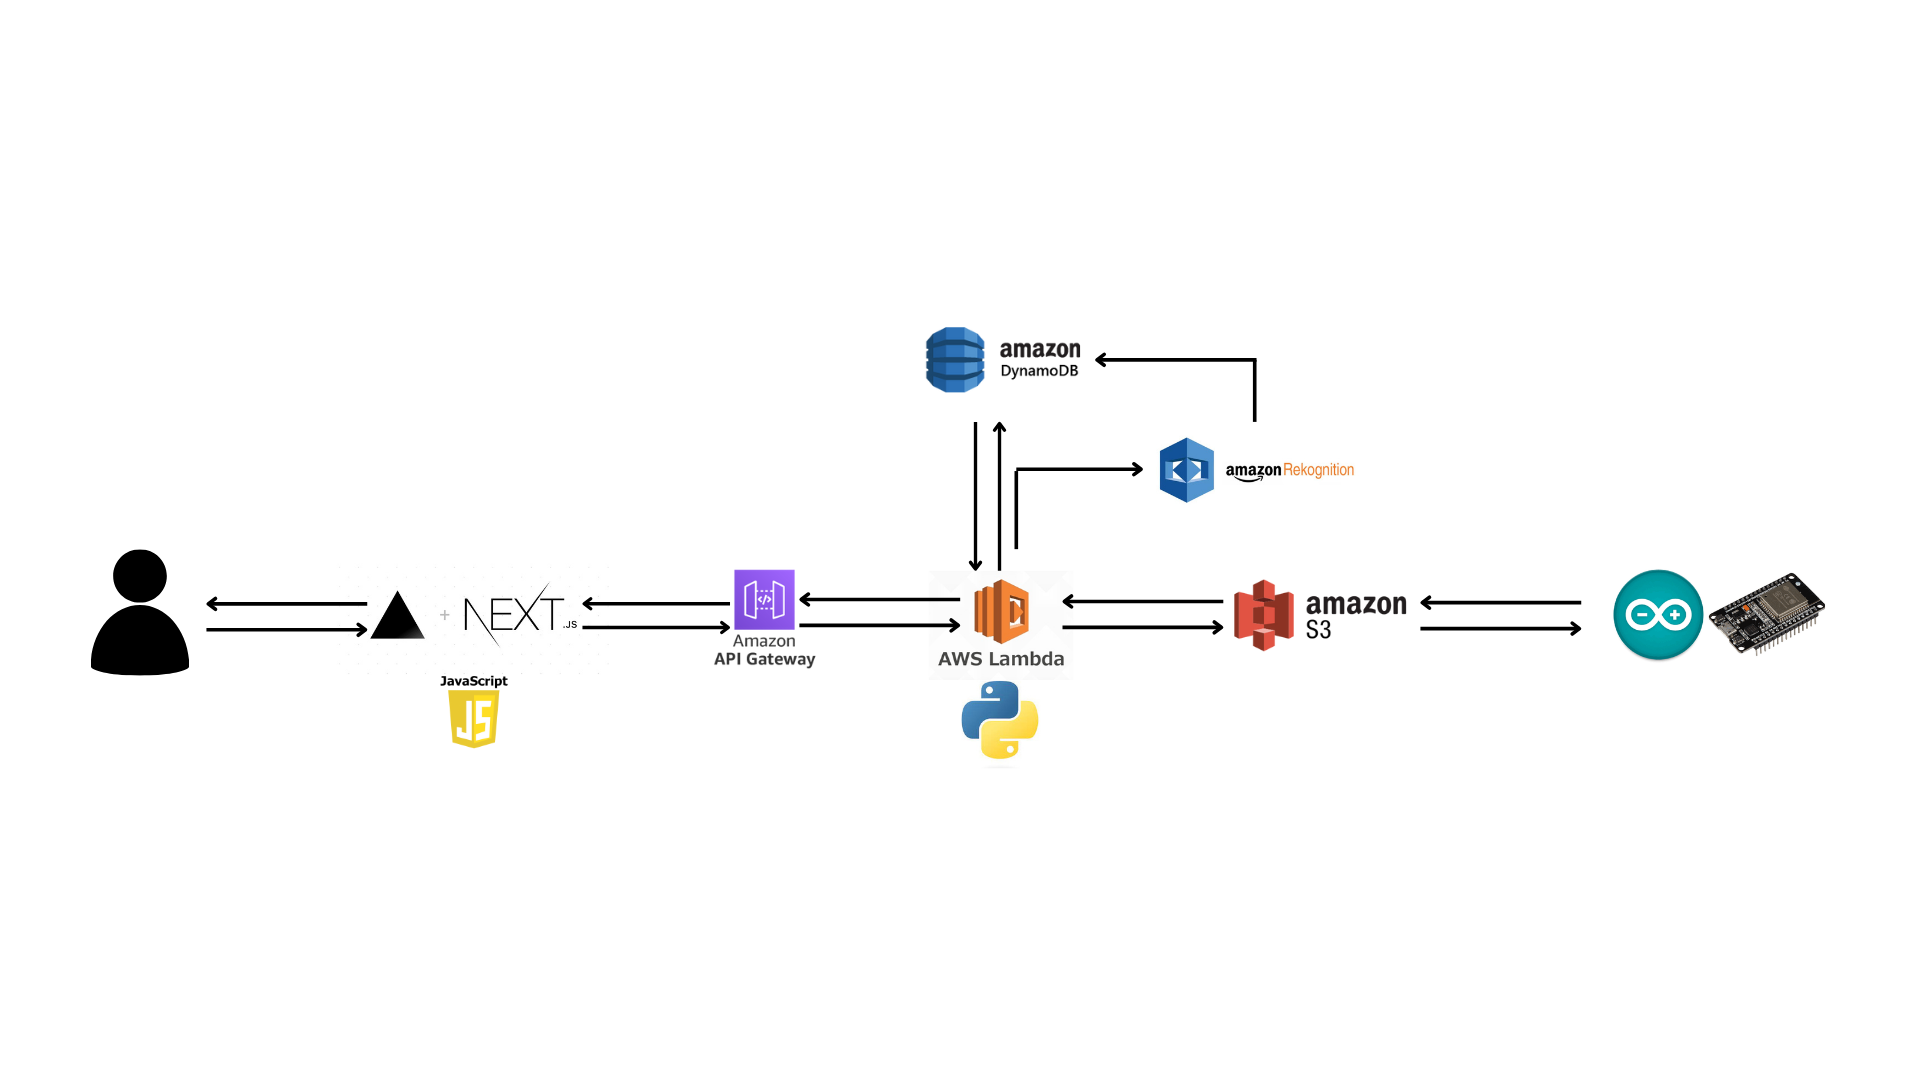
\includegraphics[width=\textwidth]{images/System Diagram.png}
\caption[System Overview]{System Overview}
\label{fig:System}
\end{figure}

\newpage
\section{การใช้งานของแอปพลิเคชัน}
ผู้ใช้งานสามารถเข้าใช้งานตัวเว็บแอปพลิเคชันได้โดยไม่ต้องทำการล็อกอินหรือยืนยันตัวตน โดยสามารถเข้าถึงข้อมูลที่แสดงอยู่บน User Interface ได้แก่ จำนวนที่นั่งที่ยังว่างอยู่ และจำนวนผู้เข้าใช้บริการในขณะนี้ 
\begin{figure}[h]
\centering
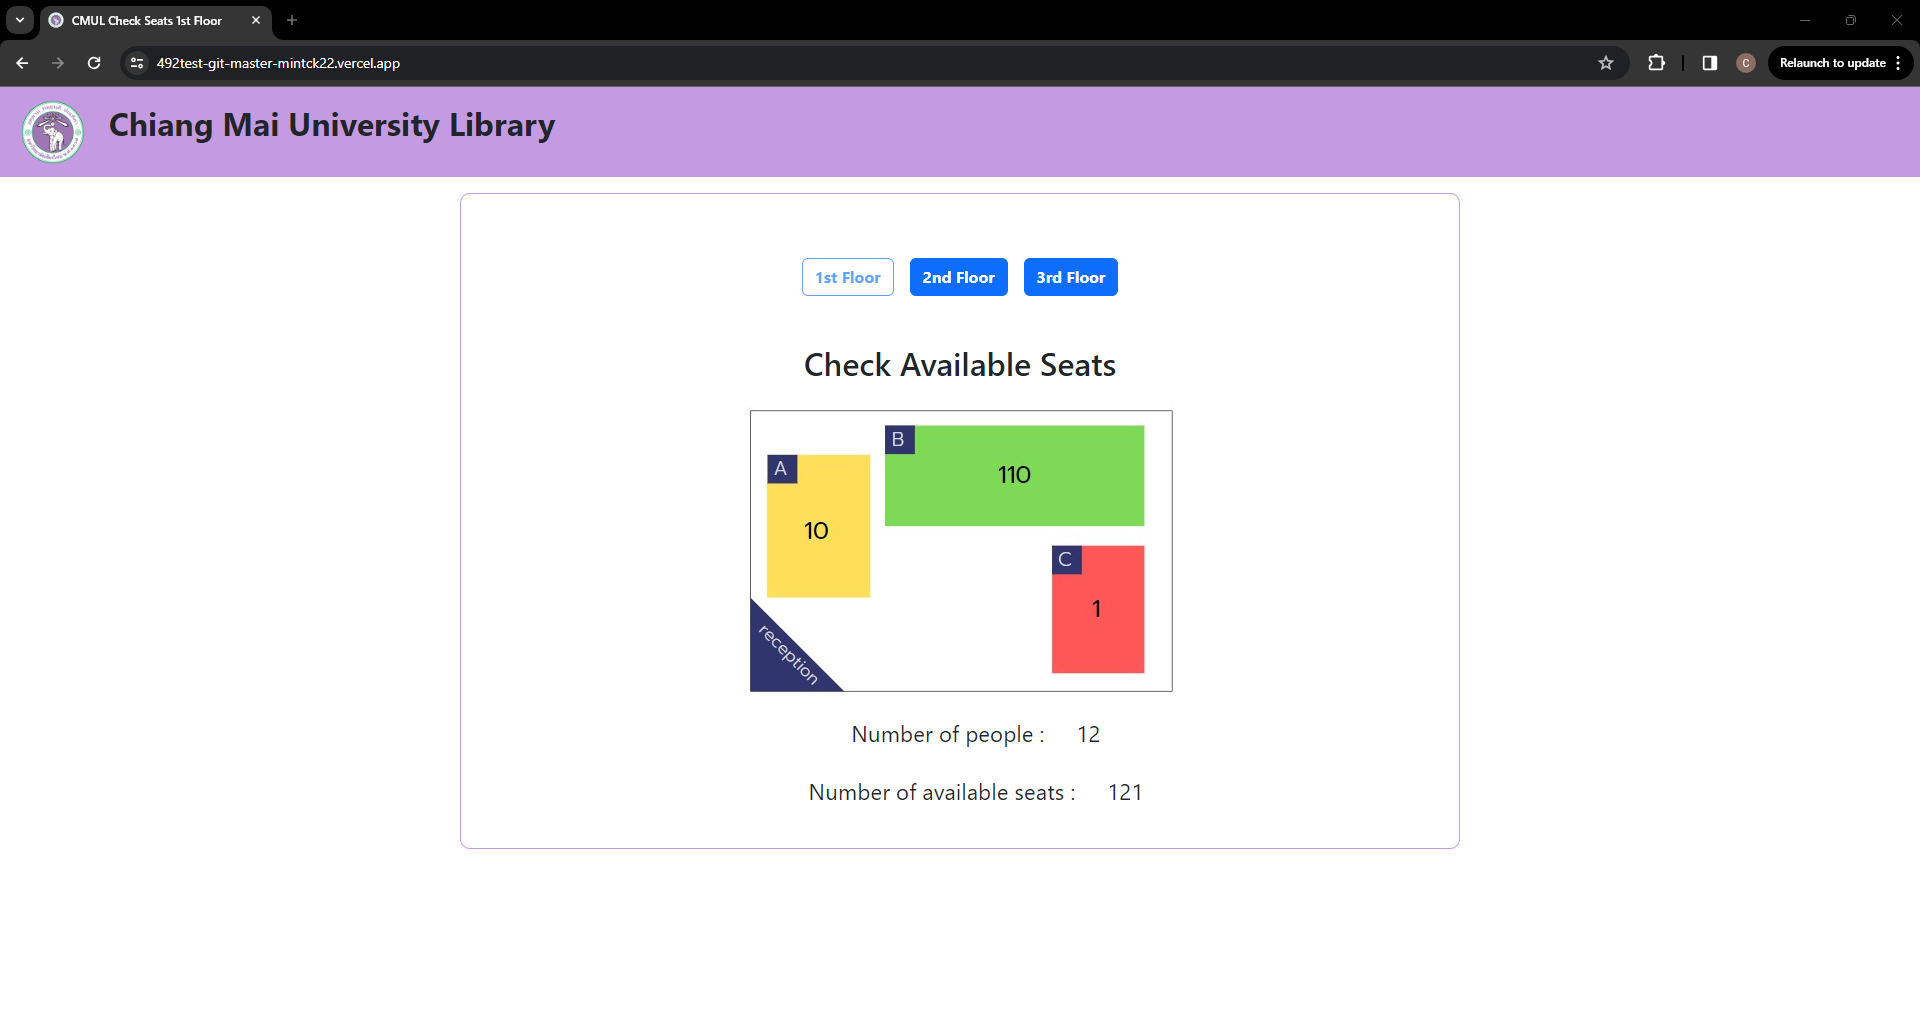
\includegraphics[width=\textwidth]{images/web1.png}
\caption[ตัวอย่างหน้าเว็บสำหรับตรวจสอบที่นั่งว่างบริเวณชั้น 1]{ตัวอย่างหน้าเว็บสำหรับตรวจสอบที่นั่งว่างบริเวณชั้น 1}
\label{fig:web1}
\end{figure}

\begin{figure}[h]
    \centering
    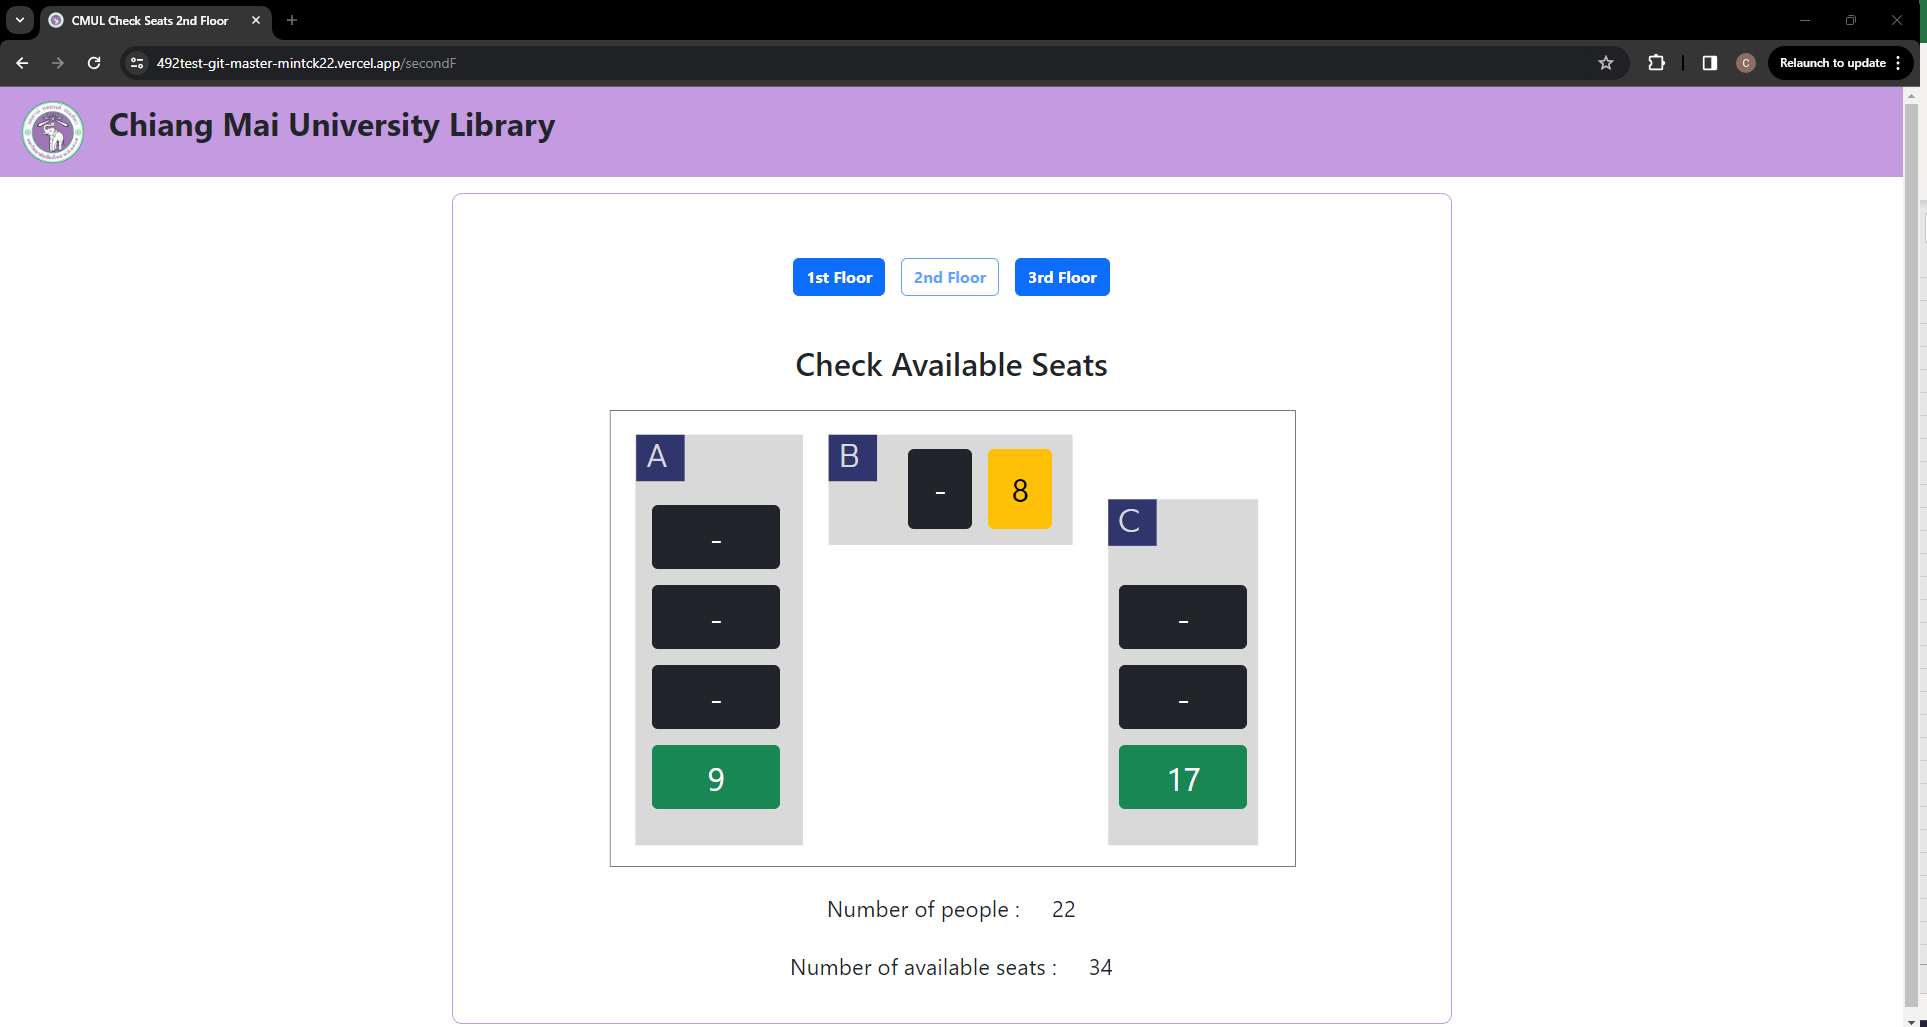
\includegraphics[width=\textwidth]{images/web2.png}
    \caption[หน้าเว็บสำหรับตรวจสอบที่นั่งว่างบริเวณชั้น 2 ที่ทำการทดสอบทั้งหมด 3 โซน]{หน้าเว็บสำหรับตรวจสอบที่นั่งว่างบริเวณชั้น 2 ที่ทำการทดสอบทั้งหมด 3 โซน}
    \label{fig:web1}
\end{figure}
โดยโซนสีเขียวจะหมายถึง มีที่นั่งที่ว่างอยู่มากกว่า 60 เปอร์เซ็นต์ของโซนนั้น สีเหลือง หมายถึง มีที่นั่งที่ว่างอยู่มากกว่า 30 เปอร์เซ็นต์แต่น้อยกว่า 60 เปอร์เซ็นต์ของโซนนั้น สีแดง หมายถึง มีที่นั่งที่ว่างอยู่น้อยกว่า 30 เปอร์เซ็นต์ของโซนนั้น ส่วนโซนสีดำ หมายถึง ไม่ได้ติดตั้งกล้องเอาไว้
